\documentclass[a4paper,12pt]{article}
\usepackage{graphicx}
\usepackage{hyperref}
\usepackage{fancyhdr}
\usepackage[a4paper, total={6in, 8in}]{geometry}
\usepackage{enumitem}
\usepackage{verbatim}




\title{\textbf{Desenvolvimento de Sistemas de Software}}
\date{Outubro 2024}

\pagestyle{plain}
\fancyhf{}
\lfoot{GitHub Repository: \href{https://github.com/LEI-DSS/DSS2425-Grupo-27}{https://github.com/LEI-DSS/DSS2425-Grupo-27}}

\begin{document}

    \begin{titlepage}
        \centering
        \vfill
        
\includegraphics[width=4cm]{512px-EEUMLOGO.png}\\
        \vspace{1.1in}
        \Large\textbf{Desenvolvimento de Sistemas de Software}\\
        Licenciatura em Engenharia Informática\\
        Universidade do Minho\\
        Grupo 27\\
        
        \textbf{Link GitHub} \href{https://github.com/LEI-DSS/DSS2425-Grupo-27}{https://github.com/LEI-DSS/DSS2425-Grupo-27}
        
      \vspace{3cm}

      
        \begin{center}
            \begin{tabular}{c c c c}
                
\includegraphics[width=0.22\textwidth]{dev1.png} & 
                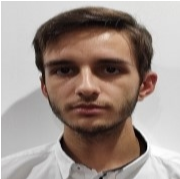
\includegraphics[width=0.22\textwidth]{dev2.png} & 
                
\includegraphics[width=0.22\textwidth]{dev3.png} & 
                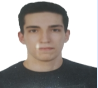
\includegraphics[width=0.22\textwidth]{dev4.png}\\
    
            David Figueiredo & Diogo Ferreira & João Carvalho & Rui Cruz \\
            (A104360) &
            (A104266) &
            (A104533) &
            (A104355)   
            \end{tabular}
        \end{center}
      \vfill
    \end{titlepage}
    % Developer Photos (4 in a row)

    \vspace{1cm}

    %\pagebreak
    %\tableofcontents
    \pagebreak
    \begin{abstract}
        Neste documento são apresentadas a modelação de domínio, o modelo de Use Cases e, parcialmente, as suas especificações. Optamos por não apresentar as especificações de todos os use cases, por existirem use cases relativos a entidades que traduzem as operações de CRUD. Isto leva a que existam use cases com comportamento semelhante, diferenciando apenas no que se está a alterar. Portanto, por uma questão de efici\^encia e desconhecimento parcial de elementos, que serão conhecidos aquando de uma implementação ou outros processos. 
    \end{abstract}

    \section{Modelo Domínio}

    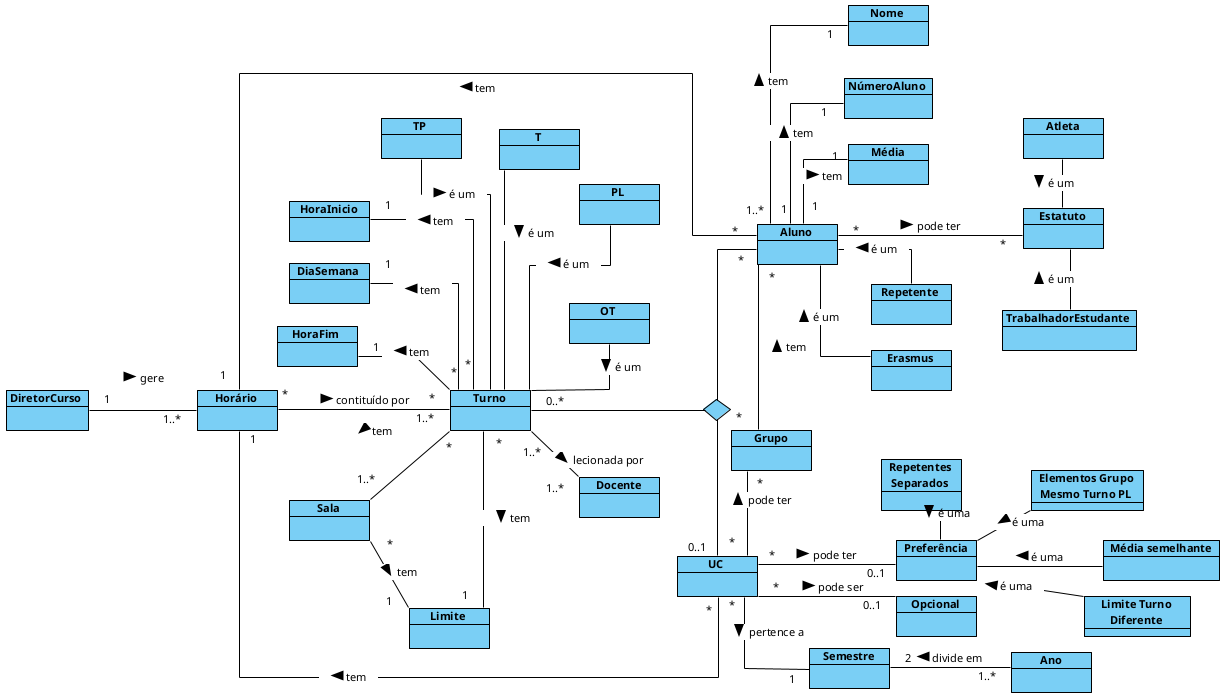
\includegraphics[width=1\textwidth]{modeloDominio2.png}\\
    \begin{center}
        \textbf{Fig.1} - Modelação de Domínio\\
    \end{center}
    \vspace{0.1in}

    \section{Diagramas de Casos de Uso}

    \section{Especificação Casos de Uso}\vspace{0.5in}
    \subsection{Importação}
    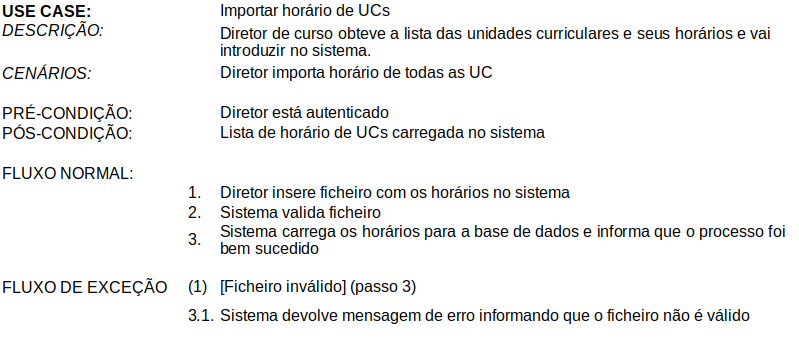
\includegraphics[width=\textwidth]{importarHorariosUC.png}\vspace{0.5in}
    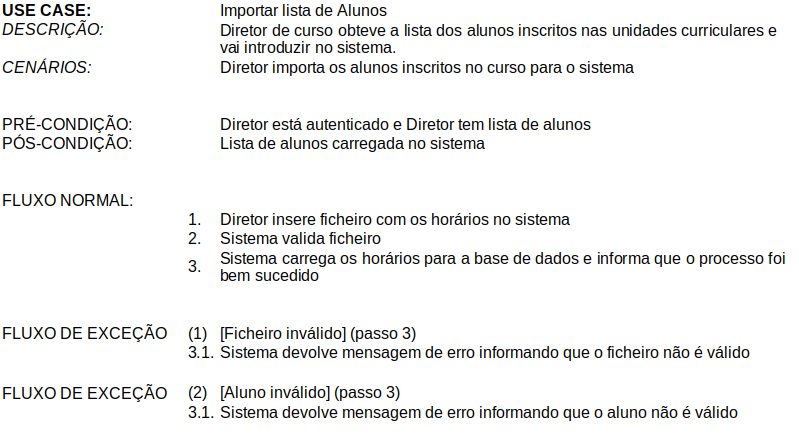
\includegraphics[width=\textwidth]{importarAlunos.png}\vspace{2cm}
    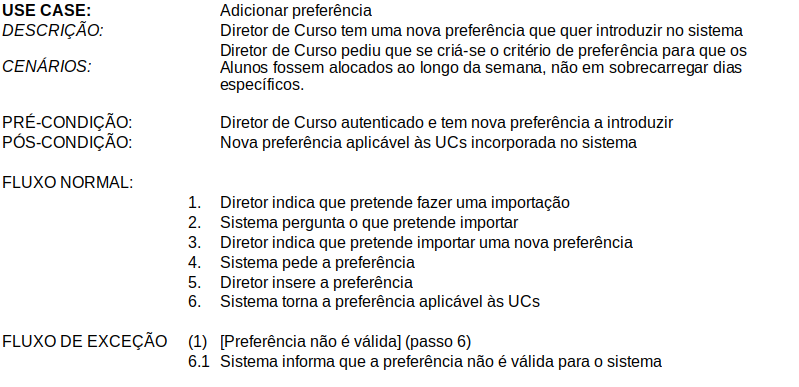
\includegraphics[width=\textwidth]{AddPrefer.png}
    \subsection{Consulta}
    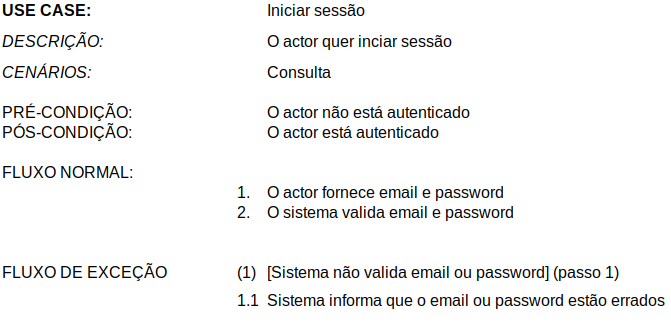
\includegraphics[width=\textwidth]{inicarSessao.png}\vspace{2cm}
    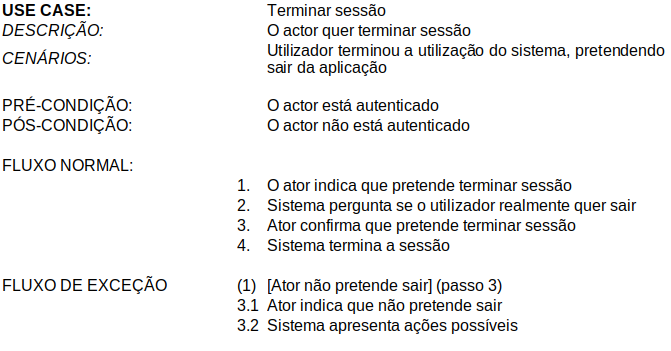
\includegraphics[width=\textwidth]{terminarsessao.png}\vspace{0.1cm}
    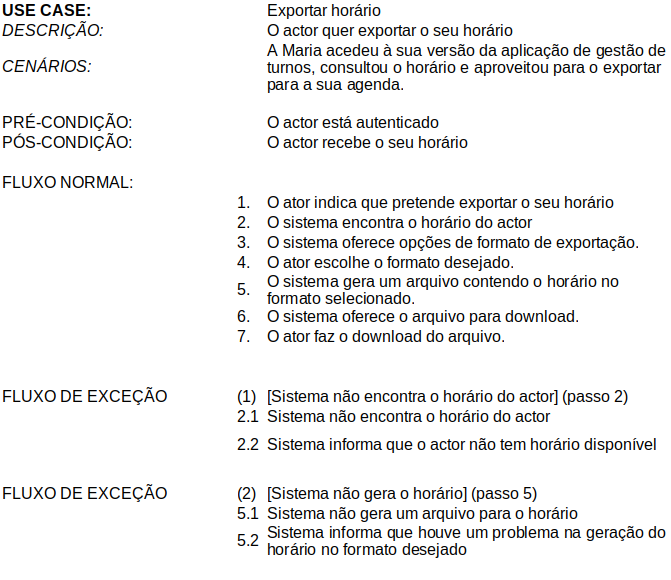
\includegraphics[width=\textwidth]{exportarHorario.png}
    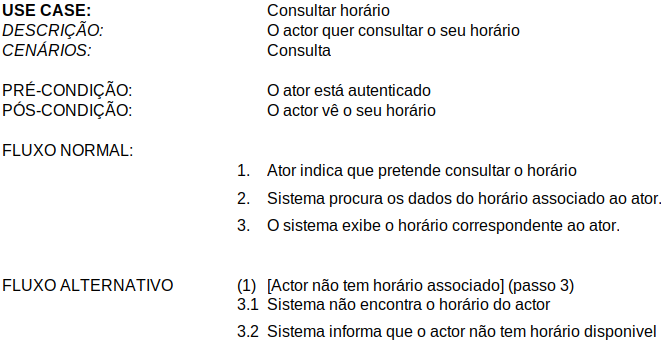
\includegraphics[width=\textwidth]{consultarHorario.png}\vspace{2cm}
    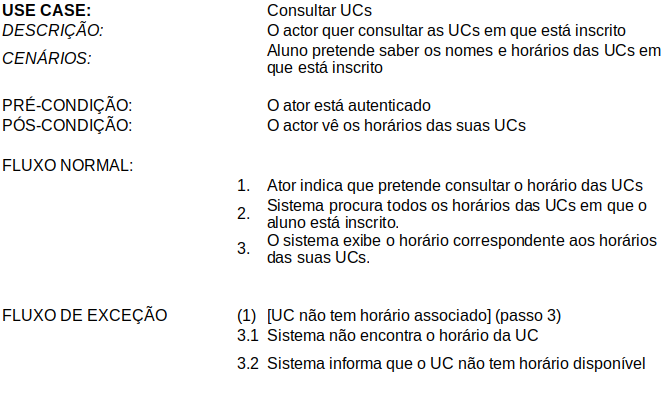
\includegraphics[width=\textwidth]{consultaUCs.png}
    \subsection{Configuração}
    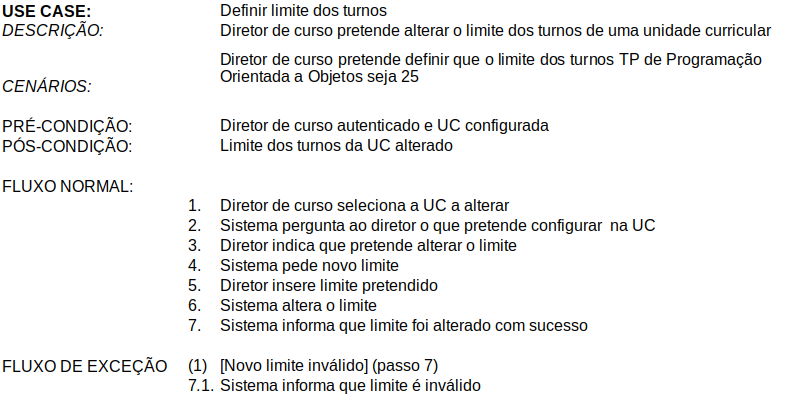
\includegraphics[width=\textwidth]{limiteTurnos.png}\vspace{2cm}
    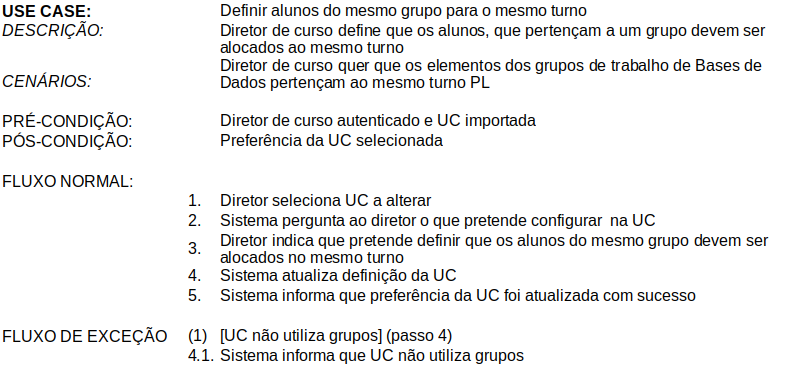
\includegraphics[width=\textwidth]{grupoTurno.png}
    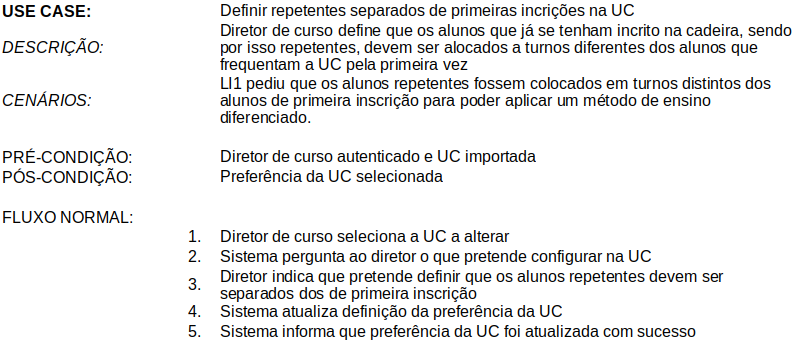
\includegraphics[width=\textwidth]{repetentes.png}\vspace{2cm}
    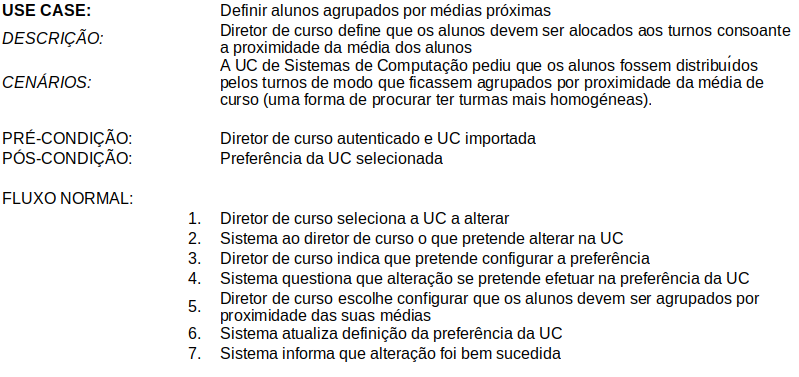
\includegraphics[width=\textwidth]{grupoMedia.png}
    \subsection{Gestão}
    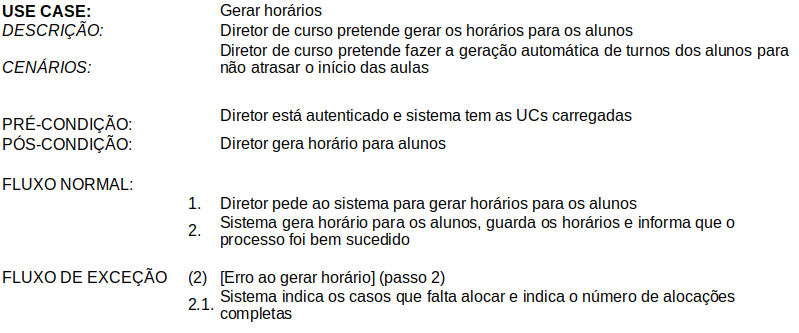
\includegraphics[width=\textwidth]{gerarHorarios.png}\vspace{0.5cm}
    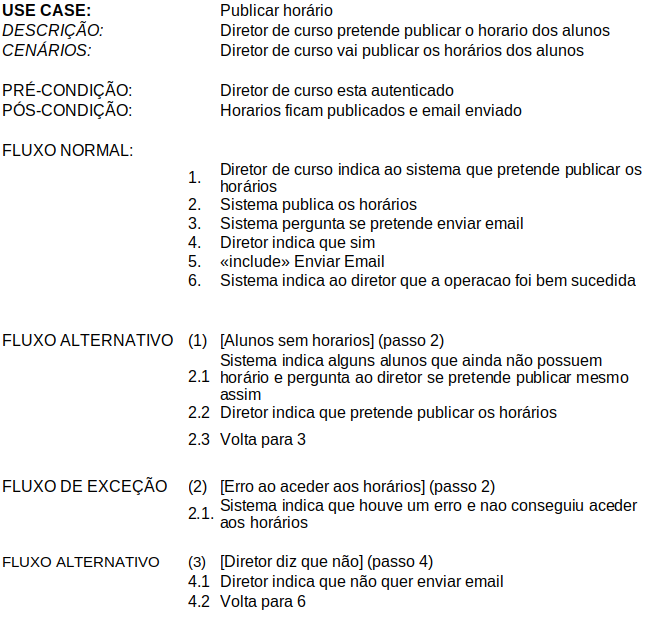
\includegraphics[width=\textwidth]{publicarHorario.png}
    
    \begin{comment}
    \section{Descrição dos resultado obtidos}

    \pagebreak
    \section{Análise de Requisitos}
    \subsection{Modelação de Domínio}
     O seguinte diagrama representa o \textbf{Modelo de Domínio} do problema apresentado. Esta representação permite compreender a realidade proposta para o problema, comunicar as ideias de forma simplificada e documentar as decisões tomadas. Além disso, engloba as entidades do problema e as relações entre elas.\\ \\
    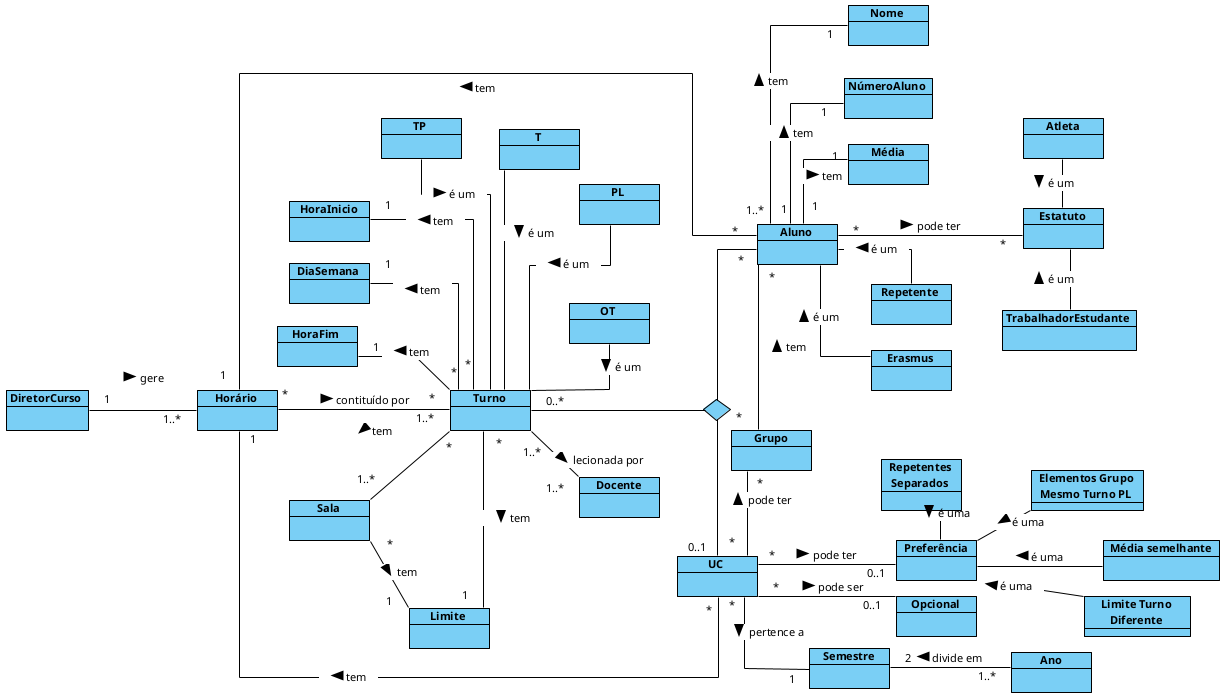
\includegraphics[width=1\textwidth]{modeloDominio2.png}\\
    \begin{center}
        \textbf{Fig.1} - Modelação de Domínio\\
    \end{center}
    \vspace{0.1in}
    Analisando o diagrama, é possível inferir o raciocínio implementado no sistema. 
    O \textbf{Diretor de Curso} é quem gere os horários dos alunos, fundamentalmente distribuindo os alunos pelos turnos.\\
    O \textbf{Horário} é constituído pelos turnos.\\
    O \textbf{Turno} é uma entidade que tem \textbf{Dia da Semana} e \textbf{Hora}. Este funciona como a representação da subdivisão operacional de uma unidade curricular. Pode ser um turno \textbf{Teórico}, \textbf{Teórico-Prático}, \textbf{Prática-Laboratorial}, \textbf{Orientação Tutória}, etc. Cada turno tem uma \textbf{Sala} atribuída, sendo que a sala contém um \textbf{Limite}. O turno possui um limite que pode ser diferente do limite da sala. \\
    A \textbf{Unidade Curricular (UC)} pertence a um \textbf{Semestre}, é lecionada por pelo menos um    \textbf{Docente}, sendo o semestre um conjunto de UCs.
    Há a possibilidade das unidades curriculares terem \textbf{Grupos} de alunos. Também é possível uma unidade curricular ter uma \textbf{Prefer\^encia} na atribuição dos alunos para os seus turnos. Existe, ainda, a escolha de uma unidade curricular poder ser \textbf{Opcional}.\\
    O \textbf{Aluno} possui um \textbf{Nome} e é identificado pelo seu \textbf{Número de Aluno}. Esta entidade possui uma \textbf{Média} que é indicador do seu desempenho ao longo do curso.
    Este também possuir um \textbf{Estatuto}, como por exemplo \textbf{Atleta} ou \textbf{Trabalhador Estudante}. As entidades \textbf{Repetentes} e \textbf{Erasmus} são tipos de alunos.\\
    Para finalizar, para cada uma unidade curricular, esta possui múltiplos alunos, cujo vínculo assenta em turnos. Não é possível a refer\^encia a alunos e unidade curricular sem a refer\^encia a, pelo menos, um turno. Reciprocamente, não é possível referir alunos e turnos sem especificar a unidade curricular.
    \subsection{Definição de requisitos}
       
    \subsubsection{Importar lista de alunos}
    \textbf{Caso de uso:} Importar lista de alunos\\
    \textbf{Descrição:} Diretor de curso obteve a lista dos alunos inscritos nas unidades curriculares e 
    vai introduzir no sistema.\\
    \textbf{Cenário:} Diretor de Curso\\
    \textbf{Pré-condição:} Diretor está autenticado e Diretor tem lista de alunos\\
    \textbf{Pós-condição:} Lista de alunos completamente carregada no sistema\\
    \textbf{Fluxo normal:} 
        \begin{enumerate}
            \item Diretor insere ficheiro no sistema
            \item Sistema valida ficheiro e carrega a lista para o sistema
            \item Sistema informa que o processo foi bem sucedido
        \end{enumerate}
    \textbf{Fluxo de exceção(1):} [Ficheiro inválido] (passo 2)
    \begin{enumerate}[label=2.\arabic*]
        \item Sistema devolve mensagem de erro informando que o ficheiro não é válido
    \end{enumerate}
    \vspace{1in}

    \subsubsection{Configurar preferências}
    \textbf{Caso de uso:} Configurar prefer\^encias de uma Unidade Curricular\\
    \textbf{Descrição:} Diretor de Curso configura que as alocações dos alunos devem ser feitas por média semelhantes para o mesmo turno\\
    \textbf{Cenário:} Diretor de Curso\\
    \textbf{Pré-condição:} Diretor de Curso está autenticado, UC presente no sistema e turnos configurados\\
    \textbf{Pós-condição:} Prefer\^encia de alocação para a UC configurada no sistema\\
    \textbf{Fluxo normal:} 
        \begin{enumerate}
            \item Diretor de Curso seleciona a UC que pretende configurar a prefer\^encia 
            \item Sistema pede operação 
            \item Diretor de Curso indica que pretende configurar a prefer\^encia de alocação
            \item Sistema exibe opções de prefer\^encias para configurar
            \item 
        \end{enumerate}
    \textbf{Fluxo de exceção(1):} [Ficheiro inválido] (passo 2)
    \begin{enumerate}[label=2.\arabic*]
        \item Sistema devolve mensagem de erro informando que o ficheiro não é válido
    \end{enumerate}
    \vspace{1in}
    \end{comment}


    
    
    %\pagebreak
    %\section{Modelação Conceptual}
    %\subsection{Diagramas de Classe}
    %\subsection{Diagramas de Sequ\^encia}

    %\pagebreak
    %\section{Solução implementada}
    %\subsection{Diagramas de Classe}
    %\subsection{Diagramas de Sequ\^encia}
    %\subsection{Diagramas de Componentes}
    %subsection{Packages}
    

\end{document}
